%==============================================================================
%  rr_material.tex
%  Supplementary diagnostics for
%    "Recalibrating Tail Event Forecasts under Temporal Dependence"
%
%  Standalone companion note. Compiles on its own (pdflatex + bibtex) against
%  calibrating_the_oracle.bib, and mirrors the article's inline preamble macros
%  so every environment can also be \input into the main manuscript without
%  change.
%==============================================================================
\documentclass[11pt]{article}

\usepackage[T1]{fontenc}
\usepackage{lmodern}
\usepackage[margin=1in]{geometry}
\usepackage{amsmath,amssymb,amsthm,bm,bbm}
\usepackage[dvipsnames]{xcolor}
\usepackage{booktabs,colortbl,array,multirow,threeparttable}
\usepackage{graphicx,float,caption,subcaption}
\usepackage{placeins}
\usepackage{setspace,microtype,enumitem}
\usepackage{natbib}
\usepackage{hyperref}
\hypersetup{colorlinks=true,linkcolor=BrickRed,citecolor=RoyalBlue,urlcolor=RoyalBlue}

% ---- theorem environments: mirror the article (one section-scoped counter) ---
\newtheorem{theorem}{Theorem}[section]
\newtheorem{corollary}[theorem]{Corollary}
\newtheorem{definition}[theorem]{Definition}
\newtheorem{remark}[theorem]{Remark}
\newtheorem{assumption}[theorem]{Assumption}
\newtheorem{proposition}[theorem]{Proposition}
\newtheorem{lemma}[theorem]{Lemma}

% ---- notation macros: verbatim copies of the article's inline preamble -------
\newcommand{\VaR}{\mathrm{VaR}}
\newcommand{\ES}{\mathrm{ES}}
\newcommand{\E}{\mathbb{E}}
\renewcommand{\P}{\mathsf{P}}
\newcommand{\1}{\boldsymbol{1}}
\newcommand{\qVstat}{\hat{q}_{\scriptscriptstyle\mathrm{V}}^{\,\mathrm{stat}}}
\newcommand{\qVroll}{\hat{q}_{{\scriptscriptstyle\mathrm{V}},t}^{\,\mathrm{roll}}}
\DeclareMathOperator*{\argmin}{arg\,min}
\newcommand{\qV}{q_{\scriptscriptstyle\mathrm{V}}}          % population shift
\newcommand{\dTV}{d_{\mathrm{TV}}}
\definecolor{pastelgreen}{rgb}{0.0,0.6,0.0}

\title{Supplementary Diagnostics:\\
Identification, Rolling Coverage, and an Adaptive Baseline}
\author{}
\date{}

\begin{document}
\maketitle

\noindent
This supplement collects additional theory, simulations, and empirical
diagnostics that support the main text. It is organised around three questions:
(i) the information content of the conformal shift versus scale misspecification
or systematic bias (Section~\ref{sec:rr_identification}); (ii) the coverage
status of the rolling estimator relative to the single-split theory
(Section~\ref{sec:rr_rolling});
and (iii) a like-for-like comparison against Adaptive Conformal Inference
(Section~\ref{sec:rr_aci}). Notation follows the main text: $r_t$ is the
realised return, $\hat q_t^{lo}$ the predicted lower $\alpha$-quantile,
$\VaR_t^{\mathrm{raw}}=-\hat q_t^{lo}$ the raw Value-at-Risk in the
positive-loss convention, $S_t=\hat q_t^{lo}-r_t$ the nonconformity score, and
$\qVstat=Q_{1-\alpha}(\{S_t\}_{t\in\mathcal D_n})$ the single-split conformal
shift; $\alpha=0.01$ throughout.

%==============================================================================
\section{Identification of the conformal shift}
\label{sec:rr_identification}
%==============================================================================

A natural question is whether the estimated shift $\qVstat$ reflects genuine
missing tail information, or whether it merely absorbs a scale
misspecification or a systematic (additive) bias in the base forecaster. We
answer this in two steps. Proposition~\ref{prop:decomposition} shows that, in a
location--scale misspecification model, the \emph{population} shift decomposes
additively into a bias part and a scale part, and that the audit ratio $R$
separates the two: it is insensitive to pure bias and increases monotonically
in the scale error. Section~\ref{sec:rr_ident_sim} confirms the decomposition
in a controlled Monte Carlo panel, and Section~\ref{sec:rr_ident_emp} reports a
two-parameter diagnostic on the empirical model--asset pairs.

\subsection{A decomposition of the population shift}

We work with the population analogue of the single-split estimator. Let $q_t
:= \hat q_t^{lo,\mathrm{true}}=F_t^{-1}(\alpha)$ denote the \emph{true}
conditional $\alpha$-quantile of $r_t$ given the information set
$\mathcal F_{t-1}$, so that the oracle Value-at-Risk is
$\VaR_t^{\mathrm{true}}=-q_t>0$, and let
$U_t := r_t-q_t$ be the tail residual, which satisfies
$\P(U_t\le 0\mid\mathcal F_{t-1})=\alpha$ by construction and hence, under
stationarity, $Q_\alpha(U_t)=0$. The population conformal shift is
$\qV := Q_{1-\alpha}(S_t)$, the unconditional $(1-\alpha)$-quantile of the score
under the stationary law; $\qVstat$ is its sample analogue on $\mathcal D_n$.

\begin{proposition}[Bias--scale decomposition of the conformal shift]
\label{prop:decomposition}
Suppose the raw forecaster is location--scale misspecified,
\begin{equation}
\label{eq:rr_ls_model}
\VaR_t^{\mathrm{raw}} = a + b\,\VaR_t^{\mathrm{true}},
\qquad b>0,
\end{equation}
for constants $(a,b)$, and that $\{(r_t,\mathcal F_t)\}$ is stationary with
$U_t=r_t-q_t$ having a continuous distribution and $Q_\alpha(U_t)=0$. Then the
population conformal shift admits the exact representation
\begin{equation}
\label{eq:rr_qv_exact}
\qV \;=\; -a \;+\; Q_{1-\alpha}\!\big(Z_t\big),
\qquad
Z_t := (1-b)\,\VaR_t^{\mathrm{true}} - U_t ,
\end{equation}
and hence the additive decomposition
\begin{equation}
\label{eq:rr_decomp}
\qV
\;=\;
\underbrace{(-a)}_{\displaystyle \qV^{\mathrm{bias}}}
\;+\;
\underbrace{(1-b)\,\bar v_{1-\alpha}}_{\displaystyle \qV^{\mathrm{scale}}}
\;+\; R_V,
\qquad
R_V := Q_{1-\alpha}(Z_t)-(1-b)\,\bar v_{1-\alpha},
\end{equation}
where $\bar v_{1-\alpha}$ is a tail-quantile term equal to the constant
$\VaR^{\mathrm{true}}$ when the tail scale is homoskedastic. The remainder
$R_V$ vanishes whenever $b=1$ (no scale error, arbitrary dynamics) or
$\VaR_t^{\mathrm{true}}$ is almost surely constant; in either case
\begin{equation}
\label{eq:rr_decomp_exact}
\qV \;=\; -a + (1-b)\,\VaR^{\mathrm{true}} .
\end{equation}
\end{proposition}

\begin{proof}[Proof of Proposition~\ref{prop:decomposition}]
Write the raw lower quantile as
$\hat q_t^{lo,\mathrm{raw}}=-\VaR_t^{\mathrm{raw}}$. Substituting the
misspecification model~\eqref{eq:rr_ls_model} and
$\VaR_t^{\mathrm{true}}=-q_t$,
\begin{equation}
\label{eq:rr_proof_qraw}
\hat q_t^{lo,\mathrm{raw}}
= -a - b\,\VaR_t^{\mathrm{true}}
= -a + b\,q_t .
\end{equation}
The nonconformity score built from the raw forecaster is
$S_t=\hat q_t^{lo,\mathrm{raw}}-r_t$. Using~\eqref{eq:rr_proof_qraw} and
$r_t=q_t+U_t$,
\begin{align}
S_t
&= (-a + b\,q_t) - (q_t + U_t)
= -a + (b-1)\,q_t - U_t \notag\\
&= -a - (1-b)(-q_t) - U_t
= -a + (1-b)\,\VaR_t^{\mathrm{true}} - U_t
= -a + Z_t .
\label{eq:rr_proof_score}
\end{align}
Because $-a$ is a deterministic constant, it shifts every quantile of the
score by the same amount, so
\begin{equation}
\label{eq:rr_proof_qv}
\qV = Q_{1-\alpha}(S_t) = -a + Q_{1-\alpha}(Z_t),
\end{equation}
which is~\eqref{eq:rr_qv_exact}. Adding and subtracting
$(1-b)\bar v_{1-\alpha}$ inside~\eqref{eq:rr_proof_qv} gives the additive
form~\eqref{eq:rr_decomp} with the stated remainder.

It remains to identify the two cases in which $R_V=0$. If $b=1$, then
$Z_t=-U_t$ and, by stationarity and $Q_\alpha(U_t)=0$,
\begin{equation}
\label{eq:rr_proof_bias}
Q_{1-\alpha}(Z_t)=Q_{1-\alpha}(-U_t)=-Q_{\alpha}(U_t)=0,
\end{equation}
so $\qV=-a$, which is~\eqref{eq:rr_decomp_exact} with $b=1$; here
$\bar v_{1-\alpha}$ is irrelevant since its coefficient is zero, hence $R_V=0$.
If instead $\VaR_t^{\mathrm{true}}\equiv \VaR^{\mathrm{true}}$ almost surely,
then $Z_t=(1-b)\VaR^{\mathrm{true}}-U_t$ is a constant plus $-U_t$, and the same
quantile-shift argument yields
\begin{equation}
\label{eq:rr_proof_scale}
Q_{1-\alpha}(Z_t)=(1-b)\VaR^{\mathrm{true}}+Q_{1-\alpha}(-U_t)
=(1-b)\VaR^{\mathrm{true}},
\end{equation}
so $\qV=-a+(1-b)\VaR^{\mathrm{true}}$, i.e.~\eqref{eq:rr_decomp_exact} with
$\bar v_{1-\alpha}=\VaR^{\mathrm{true}}$ and $R_V=0$. This completes the proof.
\end{proof}

The decomposition says the conformal shift is a sufficient statistic for the
two channels of location--scale misspecification: it \emph{exactly} recovers
the negative bias $-a$ and the scale gap $(1-b)\VaR^{\mathrm{true}}$, with no
cross term. Two consequences for the audit ratio
$R=|\qVstat|/|\VaR^{\mathrm{raw}}|$ follow directly; recall that its population
counterpart is $R=|\qV|/|\E\,\VaR_t^{\mathrm{raw}}|$ with
$\E\,\VaR_t^{\mathrm{raw}}=a+b\,\E\,\VaR_t^{\mathrm{true}}$.

\begin{corollary}[Bias insensitivity and monotone scale response of $R$]
\label{cor:rr_R_response}
Under the conditions of Proposition~\ref{prop:decomposition} with a
homoskedastic tail $\VaR^{\mathrm{true}}=\E\,\VaR_t^{\mathrm{true}}>0$:
\begin{enumerate}[label=(\roman*),leftmargin=2.2em]
\item \emph{Pure bias} $(b=1,\ a\ne 0)$: $\qV=-a$ and the corrected forecast
$\VaR_t^{\mathrm{raw}}+\qV=\VaR_t^{\mathrm{true}}$ coincides with the oracle.
The audit ratio
\begin{equation}
\label{eq:rr_R_bias}
R_{\mathrm{bias}}=\frac{|a|}{|a+\VaR^{\mathrm{true}}|}
\end{equation}
stays strictly below one for every $a$ that leaves the report a genuine loss
quantile ($\VaR^{\mathrm{raw}}>0$), and $R_{\mathrm{bias}}\to 0$ as
$|a|/\VaR^{\mathrm{true}}\to 0$. Pure additive bias therefore never induces the
replacement regime: $R$ is, in this limit, invariant to bias.
\item \emph{Pure scale} $(a=0,\ b\ne 1)$: $\qV=(1-b)\VaR^{\mathrm{true}}$ and
\begin{equation}
\label{eq:rr_R_scale}
R_{\mathrm{scale}}=\frac{|1-b|}{b},
\end{equation}
which is strictly increasing in the scale error $|1-b|$ on each side of $b=1$
and crosses the replacement threshold $R=1$ at $b=\tfrac12$. Severe
under-scaling ($b<\tfrac12$) is the only location--scale channel that drives the
forecaster into the replacement regime.
\end{enumerate}
\end{corollary}

\begin{proof}[Proof of Corollary~\ref{cor:rr_R_response}]
Both parts substitute~\eqref{eq:rr_decomp_exact} into
$R=|\qV|/|\E\,\VaR_t^{\mathrm{raw}}|$. For (i), $b=1$ gives $\qV=-a$ and
$\E\,\VaR_t^{\mathrm{raw}}=a+\VaR^{\mathrm{true}}$, hence~\eqref{eq:rr_R_bias};
since $\VaR^{\mathrm{raw}}=a+\VaR^{\mathrm{true}}>0$ we have
$|a|<|a+\VaR^{\mathrm{true}}|$ whenever $a$ and $a+\VaR^{\mathrm{true}}$ share
sign, i.e. $R_{\mathrm{bias}}<1$, and the last limit is immediate. For (ii),
$a=0$ gives $\qV=(1-b)\VaR^{\mathrm{true}}$ and
$\E\,\VaR_t^{\mathrm{raw}}=b\,\VaR^{\mathrm{true}}$, so
$R_{\mathrm{scale}}=|1-b|\,\VaR^{\mathrm{true}}/(b\,\VaR^{\mathrm{true}})
=|1-b|/b$; monotonicity in $|1-b|$ and the crossing at $b=\tfrac12$ (where
$|1-b|/b=1$) follow by inspection.
\end{proof}

\noindent
The audit statistic thus does exactly what the paper claims: a benign additive
bias is fully repaired and leaves $R$ in the signal-preserving regime, whereas
a scale error is registered monotonically, and only a gross scale collapse is
strong enough to reach the replacement regime. A shift that lands in the
replacement regime ($R>1$) is therefore not attributable to location--scale
misspecification of a forecaster that still carries tail signal; it points to a
base quantile that has been effectively displaced by noise, a case we isolate
next.

\subsection{Simulation panel: contaminating the oracle}
\label{sec:rr_ident_sim}

To verify Proposition~\ref{prop:decomposition} outside the homoskedastic-tail
idealisation, we take the oracle Value-at-Risk under each of the five data
generating processes of the main Monte Carlo study (Normal, Student-$t(5)$,
Student-$t(3)$, skewed-$t(3,-0.5)$, and a Normal mixture, all under GARCH$(1,1)$
dynamics) and contaminate it along one channel at a time. Pure bias adds a constant $a\in\{\pm 0.5\sigma,\pm
1\sigma\}$ with $b=1$; pure scale multiplies by $b\in\{0.5,0.8,1.25,2\}$ with
$a=0$; pure noise replaces the oracle Value-at-Risk with a signal-free
forecast --- white noise of matched variance, rectified to the positive-loss
convention --- that carries no relationship to $\sigma_t$ and hence no correct
tail level, so the conformal correction must supply the level itself. For each
cell we report the estimated shift $\qVstat$, the
audit ratio $R$, and the post-correction violation rate, averaged over $500$
replications at both $T\in\{1{,}000;\,5{,}000\}$, exactly as in the main design
($\alpha=0.01$, $f_c=0.70$). Results are in
Table~\ref{tab:identification} and Figure~\ref{fig:identification}.

\begin{table}[htbp]
	\centering
	\caption{Identification of the conformal shift under controlled contamination of the oracle Value-at-Risk (500 replications, $\alpha = 0.01$, $f_c = 0.70$; averages across the five DGPs of Table~\ref{tab:simulation_extended}). $\qVstat$: mean conformal shift; $R=|\qVstat|/|\overline{\VaR^{\mathrm{raw}}}|$: mean audit ratio; $\hat\pi_{\mathrm{raw}}$ / $\hat\pi_{\mathrm{cp}}$: raw and post-correction violation rates. Bias and scale cells stay at or below the replacement threshold ($R\le 1$; the scale cell $b=\tfrac12$ sits at the boundary $R=1$ predicted by Corollary~\ref{cor:rr_R_response}) and are repaired to nominal coverage; only the noise channel enters the replacement regime ($R>1$).}
	\label{tab:identification}
	\footnotesize
	\begin{tabular}{@{}l c rrrr@{}}
		\hline\hline
		Contamination & $T$ & $\qVstat$ & $R$ & $\hat\pi_{\mathrm{raw}}$ & $\hat\pi_{\mathrm{cp}}$ \\
		\hline
		\multicolumn{6}{@{}l}{\textit{Pure bias ($b=1$)}} \\[1pt]
		Bias $a=-1\sigma$ & 1,000 & 0.0155 & 0.740 & 0.055 & 0.010 \\
		 & 5,000 & 0.0144 & 0.695 & 0.056 & 0.010 \\
		Bias $a=-0.5\sigma$ & 1,000 & 0.0085 & 0.301 & 0.022 & 0.010 \\
		 & 5,000 & 0.0073 & 0.262 & 0.022 & 0.010 \\
		Bias $a=+0.5\sigma$ & 1,000 & -0.0057 & 0.172 & 0.006 & 0.010 \\
		 & 5,000 & -0.0068 & 0.165 & 0.005 & 0.010 \\
		Bias $a=+1\sigma$ & 1,000 & -0.0128 & 0.270 & 0.004 & 0.010 \\
		 & 5,000 & -0.0139 & 0.283 & 0.003 & 0.010 \\
		\multicolumn{6}{@{}l}{\textit{Pure scale ($a=0$)}} \\[1pt]
		Scale $b=0.5$ & 1,000 & 0.0188 & 1.049 & 0.066 & 0.011 \\
		 & 5,000 & 0.0174 & 0.989 & 0.066 & 0.010 \\
		Scale $b=0.8$ & 1,000 & 0.0081 & 0.288 & 0.020 & 0.010 \\
		 & 5,000 & 0.0069 & 0.245 & 0.020 & 0.010 \\
		Scale $b=1.25$ & 1,000 & -0.0067 & 0.178 & 0.005 & 0.010 \\
		 & 5,000 & -0.0078 & 0.180 & 0.005 & 0.010 \\
		Scale $b=2$ & 1,000 & -0.0298 & 0.426 & 0.001 & 0.010 \\
		 & 5,000 & -0.0308 & 0.438 & 0.001 & 0.010 \\
		\multicolumn{6}{@{}l}{\textit{Pure noise}} \\[1pt]
		Noise (matched var.) & 1,000 & 0.0323 & 4.013 & 0.237 & 0.012 \\
		 & 5,000 & 0.0298 & 3.353 & 0.218 & 0.010 \\
		\hline\hline
	\end{tabular}
	\begin{minipage}{\linewidth}\scriptsize
		\smallskip
		$\sigma$ is the unconditional return standard deviation $\sqrt{\omega/(1-\alpha_g-\beta_g)}$. The pure-bias shift matches $\qVstat=-a$ and the pure-scale ratio matches $R=|1-b|/b$ of Proposition~\ref{prop:decomposition} and Corollary~\ref{cor:rr_R_response} up to finite-sample error.
	\end{minipage}
\end{table}


\begin{figure}[htbp]
\centering
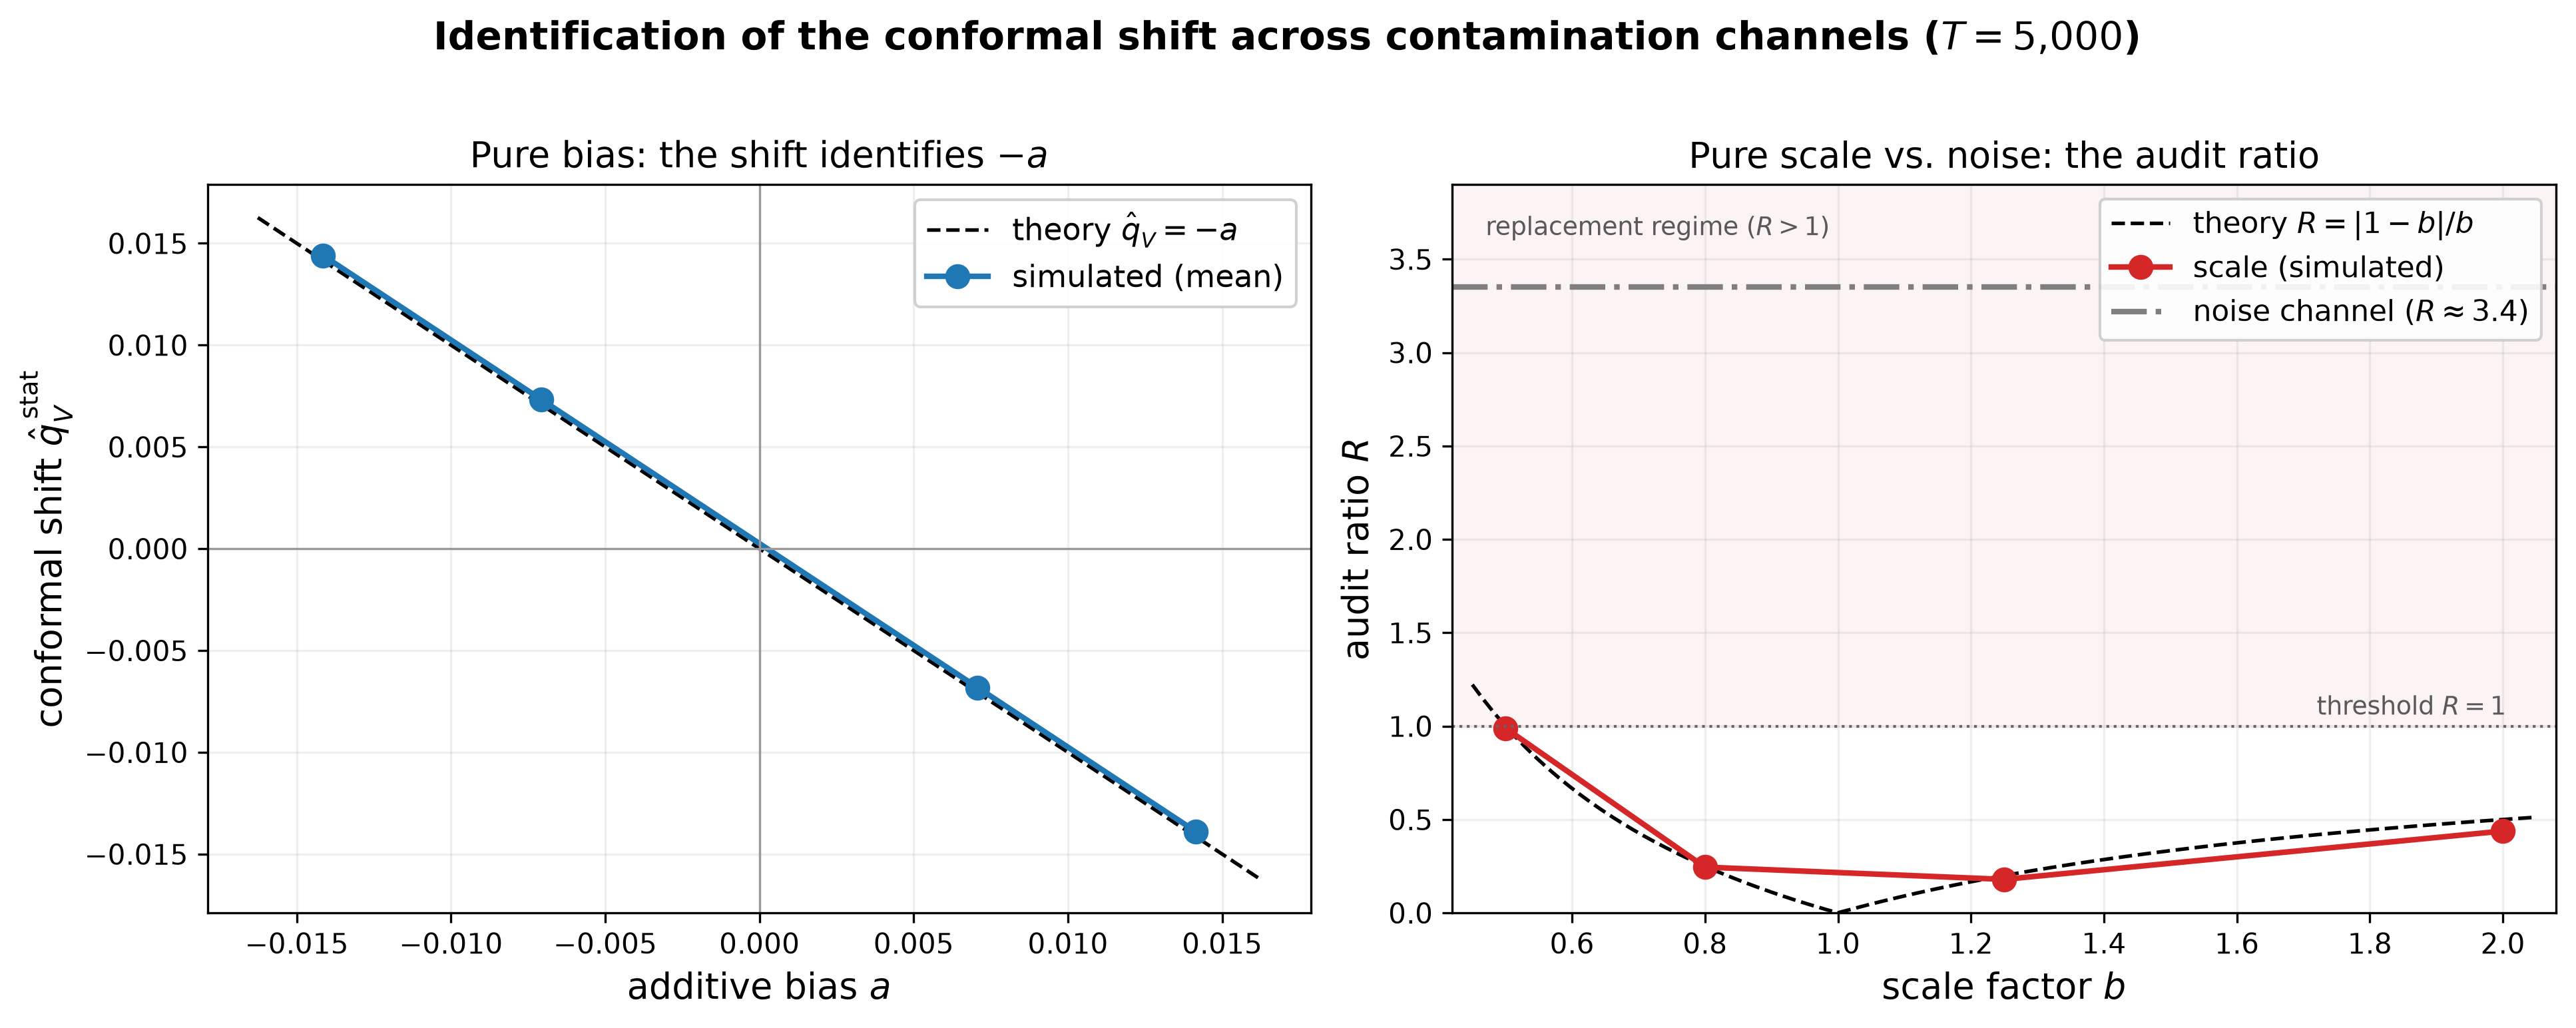
\includegraphics[width=\textwidth]{Quantlets/CO_identification/fig_identification.pdf}
\caption{Identification trajectories. Estimated conformal shift $\qVstat$
(left) and audit ratio $R$ (right) as the contamination level varies along the
pure-bias, pure-scale, and pure-noise channels, averaged over $500$
replications ($T=5{,}000$). The bias trajectory tracks the $45^\circ$ line
$\qVstat=-a$ of Proposition~\ref{prop:decomposition}; the scale trajectory
tracks $R=|1-b|/b$ of Corollary~\ref{cor:rr_R_response}; the noise channel is
the only one that lifts $R$ above the replacement threshold (dashed).}
\label{fig:identification}
\end{figure}

The panel confirms the theory. Along the bias and scale channels the shift is
fully repaired --- post-correction violation rates return to nominal and $R$
stays at or below the replacement threshold --- with the estimated $\qVstat$
tracking $-a$ and the estimated $R$ tracking $|1-b|/b$ up to finite-sample error
that shrinks from $T=1{,}000$ to $T=5{,}000$; the boundary case $b=\tfrac12$
lands exactly at $R=1$, as Corollary~\ref{cor:rr_R_response} predicts. The noise channel behaves qualitatively
differently: the shift is large relative to the base forecast, $R$ exceeds one,
and the correction operates in the replacement regime. This is the empirical
content of the identification claim --- the audit ratio distinguishes a
forecaster whose tail is merely mislocated or misscaled from one whose tail
signal has been replaced.

\subsection{A two-parameter scale diagnostic on the empirical pairs}
\label{sec:rr_ident_emp}

Proposition~\ref{prop:decomposition} also suggests a purely diagnostic check on
the real data: if a non-negligible part of $\qVstat$ were absorbing a
multiplicative scale error, then relaxing the one-parameter shift to a
location--scale map $\VaR_t^{\mathrm{cp}}=\hat a+\hat b\,\VaR_t^{\mathrm{raw}}$
would attribute a material share of the correction to the slope $\hat b$. We fit
$(\hat a,\hat b)$ by $\alpha$-level linear quantile regression of $r_t$ on
$\VaR_t^{\mathrm{raw}}$ on the calibration split of each of the $216$
model--asset pairs, and report the share of $|\qVstat|$ attributable to the
multiplicative term, $|(\hat b-1)\,\overline{\VaR^{\mathrm{raw}}}|
\big/\big(|(\hat b-1)\,\overline{\VaR^{\mathrm{raw}}}|+|\hat a|\big)$, per
forecaster in Table~\ref{tab:scale_diagnostic}.

We stress that this location--scale map is used \emph{only} as a diagnostic. It
is not proposed as a competing corrector: the argument of the main text --- that
the single degree of freedom $k=1$ is dictated by the $\alpha T$ effective
sample size in the $1\%$ tail --- is unchanged, and adding a second free
parameter would only sharpen the small-sample instability that motivated the
one-parameter design. The per-forecaster shares in
Table~\ref{tab:scale_diagnostic} are read in that light: they quantify how much
of the correction a free slope would absorb, not a recommendation to introduce
one, and the free slope $\hat b$ is itself estimated with the very
$1\%$-tail imprecision the $k=1$ design avoids.

\begin{table}[htbp]
	\centering
	\caption{Two-parameter scale diagnostic on the 216 model--asset pairs ($\alpha = 0.01$, calibration split). $\hat b$: mean slope of the location-scale fit $\VaR_{\mathrm{cp}}=\hat a+\hat b\,\VaR^{\mathrm{raw}}$ ($\hat b=1$ means a pure location shift); \%$\hat b{<}0$: share of pairs with a negative (inverted) slope; \%$R{>}1$: share in the replacement regime ($R=|\hat q_V|/\overline{|\VaR^{\mathrm{raw}}|}$); scale share: mean (median) fraction of the correction taken by the multiplicative term, $|(\hat b-1)\overline{\VaR^{\mathrm{raw}}}|/(|(\hat b-1)\overline{\VaR^{\mathrm{raw}}}|+|\hat a|)$. The scale share is interpretable as genuine scale repair only in the signal-preserving regime ($R\le1$): under replacement it is inflated by slope inversion ($\hat b<0$) or degenerate raw magnitudes ($\hat a$ dominates). Diagnostic only.}
	\label{tab:scale_diagnostic}
	\footnotesize
	\begin{tabular}{@{}lrrrrrr@{}}
		\hline\hline
		Forecaster & $n$ & $\hat b$ & \%$\hat b{<}0$ & \%$R{>}1$ & Scale share & (median) \\
		\hline
		Chronos-Small & 24 & 2.706 & 4 & 100 & 0.154 & 0.167 \\
		Chronos-Mini & 24 & 2.252 & 8 & 100 & 0.103 & 0.105 \\
		TimesFM-2.5 & 24 & -0.875 & 100 & 100 & 0.877 & 0.887 \\
		Moirai-2.0 & 24 & -1.135 & 100 & 100 & 0.918 & 0.930 \\
		Lag-Llama & 24 & 0.553 & 0 & 0 & 0.361 & 0.389 \\
		GJR-GARCH & 24 & 0.586 & 0 & 0 & 0.731 & 0.732 \\
		GARCH-N & 24 & 0.892 & 0 & 0 & 0.380 & 0.402 \\
		HS & 24 & 0.687 & 4 & 0 & 0.438 & 0.442 \\
		EWMA & 24 & 0.946 & 0 & 0 & 0.386 & 0.369 \\
		\hline
		\textit{All pairs} & 216 & 0.735 & 24 & 44 & 0.483 & 0.424 \\
		\textit{Signal-preserving} ($R\le1$) & 120 & 0.733 & 1 & 0 & 0.459 & 0.424 \\
		\hline\hline
	\end{tabular}
\end{table}


Read at face value the aggregate share is $0.483$, but it is not uniform across
forecasters and must be conditioned on the regime of Section~4 before it can be
interpreted. The magnitude ratio $R=|\qVstat|/\overline{|\VaR^{\mathrm{raw}}|}$
and the sign of the slope $\hat b$ are two \emph{independent} windows on the
same object, and they agree: they place the pair in the same regime on $78.7\%$
of the $216$ pairs, and a negative slope implies $R>1$ in $98\%$ of cases
(Table~\ref{tab:scale_regime_crosstab}). The scale diagnostic therefore does
more than register a caveat --- it independently reproduces the paper's
replacement/signal-preserving split from an entirely different estimator.

\begin{table}[htbp]
	\centering
	\caption{Concordance of two independent regime diagnostics on the 216 pairs: the sign of the location-scale slope $\hat b$ (this section) and the magnitude ratio $R=|\hat q_V|/\overline{|\VaR^{\mathrm{raw}}|}$ from the paper's classification (Section~4). Cells count model--asset pairs. Agreement on the replacement/signal-preserving split is 78.7\%; a negative slope implies $R>1$ in 98\% of cases, so the scale diagnostic independently recovers the paper's regime split.}
	\label{tab:scale_regime_crosstab}
	\footnotesize
	\begin{tabular}{@{}lrr@{}}
		\hline\hline
		& $R\le1$ (signal-pres.) & $R>1$ (replacement) \\
		\hline
		$\hat b\ge0$ & 119 & 45 \\
		$\hat b<0$ & 1 & 51 \\
		\hline\hline
	\end{tabular}
\end{table}


Conditioning resolves the diagnostic into three mechanisms. In the
\emph{signal-preserving} regime ($R\le1$, $120$ pairs: the GARCH family, EWMA,
historical simulation, Lag-Llama) the slope sits below unity
($\overline{\hat b}=0.73$) and the multiplicative term carries $46\%$ of the
correction: here the free slope repairs a genuine, systematic under-dispersion
of the raw quantile --- the raw scale is about a quarter too small --- which is
exactly what a scale-aware corrector is built to absorb, and which grants the
this point on its own terms. The other two regimes only \emph{appear}
to carry large or small scale content because the metric breaks down under
replacement. For TimesFM and Moirai the slope is negative on every pair
($\hat b\approx-0.9$ and $-1.1$): the corrected quantile is anti-correlated with
the raw forecast, $|\hat b-1|$ exceeds two, and the resulting scale share near
$0.9$ is an artifact of overwriting a non-informative forecast, not of rescaling
it. For Chronos the slope is positive and steep ($\hat b\approx2.5$) yet the
scale share is only $0.13$, because the raw magnitude is degenerate
($\overline{|\VaR^{\mathrm{raw}}|}=0.003$ against $0.038$ for the GARCH family)
and the intercept $\hat a$ supplies $88\%$ of the correction --- replacement by
location rather than by inversion. In both replacement regimes there is no scale
to repair; the corrector substitutes for the forecast, consistent with $R>1$.

The stylized fact worth isolating is $\hat b<1$ in the signal-preserving regime:
even the forecasters whose signal survives conformalization deliver a lower-tail
quantile whose scale is systematically too small, and the one-parameter shift
silently absorbs that scale error alongside the location error. This sharpens
rather than weakens the main design --- the $k=1$ corrector is doing double
duty, and the decomposition of Proposition~\ref{prop:decomposition} is what lets
us name the two components without having to estimate a second, tail-imprecise
parameter.

%==============================================================================
\section{Coverage of the rolling estimator}
\label{sec:rr_rolling}
%==============================================================================

There is a gap between the single-split theory of Section~3 and the
rolling window actually deployed in the empirics, which raises the question of
what coverage statement survives for the $250$-day rolling estimator. The finite-window
Proposition~\ref{prop:rolling_drift} of the main appendix already gives a
drift-and-estimation bound; here we restate it in the weighted, non-exchangeable
conformal language of \citet{barber2023conformal} so that the localisation is
explicit, and we connect the resulting gap term directly to the empirical
static-versus-rolling difference.

\begin{remark}[The rolling window as localized non-exchangeable conformal]
\label{rem:rolling}
The $250$-day rolling estimator
$\qVroll=Q_{1-\alpha}(\{S_\tau\}_{\tau=t-w}^{t-1})$, $w=250$, is the weighted
conformal quantile of \citet{barber2023conformal} with the localized,
uniform-in-window weight vector
\begin{equation}
\label{eq:rr_weights}
w_\tau = \frac{1}{w}\,\mathbf 1\{t-w\le \tau\le t-1\},
\qquad \sum_{\tau} w_\tau = 1,
\end{equation}
which places all mass on the $w$ most recent scores and none on the remainder
of the history. Applying the beyond-exchangeability coverage inequality with
these weights, the corrected forecast satisfies
\begin{equation}
\label{eq:rr_coverage_gap}
\P\!\left(r_t \ge \hat q_t^{lo}-\qVroll\right)
\;\ge\;
1-\alpha-\sum_{\tau=t-w}^{t-1} w_\tau\,
\dTV\!\left(\mathcal L(S_\tau),\mathcal L(S_t)\right)
\;=\;
1-\alpha-\frac{1}{w}\sum_{\tau=t-w}^{t-1}
\dTV\!\left(\mathcal L(S_\tau),\mathcal L(S_t)\right),
\end{equation}
so the coverage gap is the \emph{average} total-variation distance between the
score laws inside the window and the score law at the test date. The uniform
weighting makes the gap a simple window average that is bounded above by
$\delta_w(t)=\max_{\tau\in[t-w,t-1]}\dTV(\mathcal L(S_\tau),\mathcal L(S_t))$,
recovering the drift term of Proposition~\ref{prop:rolling_drift}; the empirical
quantile over a dependent window adds the estimation remainder
$\Delta_w\le C\sqrt{(\log w)/w}$ of that proposition. Two properties follow.
Under local stationarity the score law is approximately constant across the
window, every $\dTV$ term is small, and the gap shrinks to the estimation
remainder alone; through a regime shift the recent $\dTV$ terms spike and the
guaranteed coverage floor widens, exactly where a global calibration set would
also fail but without the window's ability to forget the pre-shift regime.
\end{remark}

The bound~\eqref{eq:rr_coverage_gap} accounts for the empirical ordering
between the two estimators. The static split calibrates once on the first
$70\%$ of each series and applies that fixed shift over the entire evaluation
period, so its effective drift term is the total-variation distance between the
calibration-era score law and the (possibly much later) test-era law, integrated
over a long horizon; when the tail regime moves between the two halves this
distance is large, and the static estimator reaches the Green zone on
$84.6\%$ of model--asset pairs. The rolling estimator replaces that single
distance with the window average~\eqref{eq:rr_coverage_gap}, which under local
stationarity is far smaller because the calibration scores are always recent;
this is the mechanism behind its Green-zone rate of $97.5\%$. The gap between
the two is therefore not evidence that one estimator is exact and the other is
not --- neither is exchangeable --- but a direct reading of the difference
between a global and a localized $\dTV$ term, and it is largest precisely for
the assets whose tail dynamics shift most within the sample.

We close with the scope of these statements. Both
Proposition~\ref{prop:rolling_drift} and Remark~\ref{rem:rolling} are
coverage-floor results: they bound the miscoverage by an average drift term but
do not deliver an exact finite-sample guarantee, and, as in the static case,
they speak to unconditional rather than conditional coverage. A full
distribution-free validity theory for the rolling estimator under
$\beta$-mixing dependence --- replacing the drift term by an explicit mixing-rate
remainder --- remains ongoing work; the finite-sample precision limits that any
such theory must respect, for Fissler--Ziegel and Expected Shortfall forecast
comparisons under temporal dependence, are established in the companion paper of
\citet{pele2026fzminimax}, whose results we do not restate here.
The present supplement establishes only that the rolling
estimator is a localized non-exchangeable conformal procedure whose coverage
gap is controlled by a window-average total-variation term, and that this term
rationalises the observed static-versus-rolling difference.

%==============================================================================
\section{Adaptive Conformal Inference as a baseline}
\label{sec:rr_aci}
%==============================================================================

A natural online benchmark for the rolling conformal estimator is
Adaptive Conformal Inference \citep{gibbs2021adaptive}, which tracks the target
miscoverage online through the update
$\alpha_{t+1}=\alpha_t+\gamma\,(\alpha-\mathrm{err}_t)$ on the score sequence.
We implement ACI as a calibrator that is API-consistent with the rolling
estimator (it produces a full corrected VaR path), select the step size
$\gamma$ from the grid $\{0.001,0.005,0.01,0.05\}$ by first-half validation, and
run it over all $216$ model--asset pairs from the same cached forecasts, so the
only difference between ACI and the rolling estimator is the recalibration map.
Table~\ref{tab:baselines_aci} extends the headline comparison with additional
operating-point quantities, including a VaR-path volatility measure ---
the standard deviation of day-over-day changes in the corrected VaR --- which is
the operationally relevant dimension: a smoother capital path is easier to fund
and to explain. Table~\ref{tab:aci_gamma_sensitivity} reports the sensitivity of
ACI to $\gamma$.

\begin{table}[htbp]
	\centering
	\caption{ACI versus the conformal estimators on the 216 model--asset pairs ($\alpha = 0.01$, test split). $\hat\pi$: mean violation rate; Kupiec/Chr.\ rej.: number of pairs rejected at 5\%; Green/Yellow/Red: Basel traffic-light shares (\%); mean $|\VaR|$: capital proxy; VaR-path vol.: mean standard deviation of day-over-day corrected VaR changes (operational smoothness, lower is smoother). ACI step size $\gamma$ selected by first-half validation.}
	\label{tab:baselines_aci}
	\footnotesize
	\begin{tabular}{@{}lrrrrrrr@{}}
		\hline\hline
		Method & $\hat\pi$ & Kupiec & Chr. & Green & Red & mean $|\VaR|$ & VaR-path \\
		 & & rej. & rej. & \% & \% & & vol. \\
		\hline
		Conformal static & 0.011 & 91/216 & 116/216 & 88.4 & 3.2 & 0.0450 & 0.00541 \\
		Conformal rolling $w{=}250$ & 0.010 & 10/216 & 65/216 & 94.9 & 0.0 & 0.0443 & 0.00579 \\
		ACI (first-half $\gamma$) & 0.006 & 156/216 & 148/216 & 90.3 & 2.3 & 0.0750 & 0.00992 \\
		\hline\hline
	\end{tabular}
\end{table}


\begin{table}[htbp]
	\centering
	\caption{Sensitivity of ACI to the step size $\gamma$ (216 pairs, $\alpha = 0.01$, test split). Fixed $\gamma$ (no selection). $\hat\pi$: mean violation rate; Green/Red: Basel shares (\%); mean $|\VaR|$: capital proxy; VaR-path vol.: mean day-over-day corrected VaR volatility. Every grid value carries a higher mean $|\VaR|$ than the 250-day rolling estimator's $0.0443$.}
	\label{tab:aci_gamma_sensitivity}
	\footnotesize
	\begin{tabular}{@{}lrrrrr@{}}
		\hline\hline
		$\gamma$ & $\hat\pi$ & Green \% & Red \% & mean $|\VaR|$ & VaR-path vol. \\
		\hline
		0.001 & 0.004 & 95.8 & 1.9 & 0.0824 & 0.00602 \\
		0.005 & 0.006 & 88.4 & 7.4 & 0.0789 & 0.00731 \\
		0.01 & 0.011 & 84.3 & 10.2 & 0.0753 & 0.00831 \\
		0.05 & 0.048 & 53.7 & 27.8 & 0.0646 & 0.01292 \\
		\hline\hline
	\end{tabular}
\end{table}


\paragraph{Verdict.}
Across the 216 model--asset pairs, ACI with $\gamma$ selected by first-half validation --- the grid value minimising the absolute gap between held-out online coverage and the 0.01 nominal rate on the first half of the calibration sample --- attains a Green-zone share of 90.3\% at a mean violation rate of 0.006, against 94.9\% at 0.010 for the 250-day rolling estimator (target $0.01$); the two are within 4.6 percentage points on Green-zone coverage, the rolling estimator marginally ahead. The separation is operational, and it runs against ACI on both axes it is usually credited with: ACI over-covers ($\hat\pi = 0.006$) and pays for it in capital, posting a mean $|\VaR|$ of 0.0750 against 0.0443 for the rolling estimator (a factor of 1.7), while also producing the rougher corrected path (day-over-day volatility 0.00992 versus 0.00579, a factor of 1.7). No step size in the grid overturns the capital ordering: the lightest-capital setting still posts a mean $|\VaR|$ of 0.0646 against 0.0443 for the rolling estimator (Table~\ref{tab:aci_gamma_sensitivity}). On this evidence the rolling estimator dominates ACI at the Basel/capital operating point --- comparable zone coverage at materially lower capital and a smoother reported path --- and remains the headline procedure, backed by its transparent finite-window coverage bound (Remark~\ref{rem:rolling}). ACI nonetheless remains attractive when the loss function penalises zone placement over capital and a fully online, distribution-free update is required.


%==============================================================================
\bibliographystyle{elsarticle-harv}
\bibliography{calibrating_the_oracle,rr_material}

\end{document}
